\documentclass{projdoc}

\title{Software Design}

\begin{document}
\tablestables
\newpage

\section{Introduction}

This document outlines the design and development process of the cr\^epe game engine,
detailing the key decisions made during its creation. The primary goal of this engine
is to offer a streamlined, Unity-like experience tailored for developing 2D games
similar to Jetpack Joyride.

The cr\^epe engine is designed to ease the transition for developers familiar with
Unity, ensuring minimal friction when switching platforms. Our aim is to preserve
many of Unity’s core features while introducing a lightweight and open-source
alternative, licensed under the MIT License.

The engine is primarily aimed at indie developers who have prior experience with
Unity and are looking for a flexible, cost-effective solution with familiar
workflows.

\section{Overview}

\subsection{Core}

\subsection{Patterns}

\section{Design}
\subsection{Game Loop}
\subsubsection{Problem statement:}
The game loop is integrated into the engine to simplify development and minimize timing issues. By embedding the game loop within the engine, uniform execution of engine systems is ensured.
Two separate update functions are employed: a fixed-time update with a consistent time delay per call is used for game logic and physics, ensuring predictable behavior regardless of fluctuations in frame rates.
This approach decouples physics calculations from the frame rate, allowing consistent behavior across different hardware configurations.
\subsubsection{Design:}
As illustrated in Figure \ref{gameloop-flow}, the game loop continues to call the fixed update function as long as sufficient time is available.
Delta time, calculated using the time between the start of the last frame and the current frame, is used to measure the duration of each frame. This value is converted into a time-based unit, enabling other systems or game developers to create behavior independent of frame rate.

Rendering and animations are handled separately on a per-frame basis. A delay, in conjunction with the delta time calculation, is applied to maintain consistent visual behavior, even when frame rates vary. This separation of game logic from rendering ensures that both simulation accuracy and visual fluidity are optimized.
As seen in figure Figure \ref{gameloop-class} to access the deltaTime anywhere in the system a timerClass is created using a singleton desing pattern which ensures only one instance of the class is created; the gameloop updates the timing and delta time of this class to ensure it is accurate.
The gameloops two main functions are the setup() and loop(). The first is called when the game starts and handles all startup procedures this function only runs once.
The loop() function keeps looping as long as the game is running. Within this function are the functions: processInputs for handling user input(mouse,keyboard,other controllers),fixed update,frame update and render function.
\begin{figure}
	\centering
	\includepumldiag{img/gameloop-flow.puml}
	\caption{Gameloop Flowchart Diagram} \label{gameloop-flow}
\end{figure}

\begin{figure}
	\centering
	\includepumldiag{img/gameloop-class.puml}
	\caption{Gameloop Flowchart Diagram} \label{gameloop-class}
\end{figure}
\subsection{Event system}
\subsubsection{Problem statement:}
\subsubsection{Problem Statement:}
The game engine utilizes the Entity-Component-System (ECS) architecture, where components store data, and systems process that data to apply changes. Each system is responsible for managing a specific domain, such as physics in the physics system and rendering in the rendering system. To facilitate communication between systems without introducing direct dependencies, a method of inter-system communication is required to maintain loose coupling.

Additionally, a mechanism that allows one object's trigger to elicit responses from multiple other objects is beneficial for game developers, providing greater flexibility in designing interactions within the game.

\subsubsection{Design:}
The solution to the aforementioned problems is an event system that facilitates communication between systems and utilizes BehaviorScripts to handle various types of events. The event system includes several pre-defined events, all derived from a parent Event class, capable of handling user input and application-level events, such as window resizing.

Furthermore, a specific event is designated for the collision handler within the physics system, which can be triggered when two objects collide. The event system also allows developers to create custom events, such as "onPlayerDeath," and assign callback functions that execute when the event is triggered.

When such an event occurs, the EventManager calls the assigned callback function, executing the associated code to handle the event's consequences
\begin{figure}
    \centering
    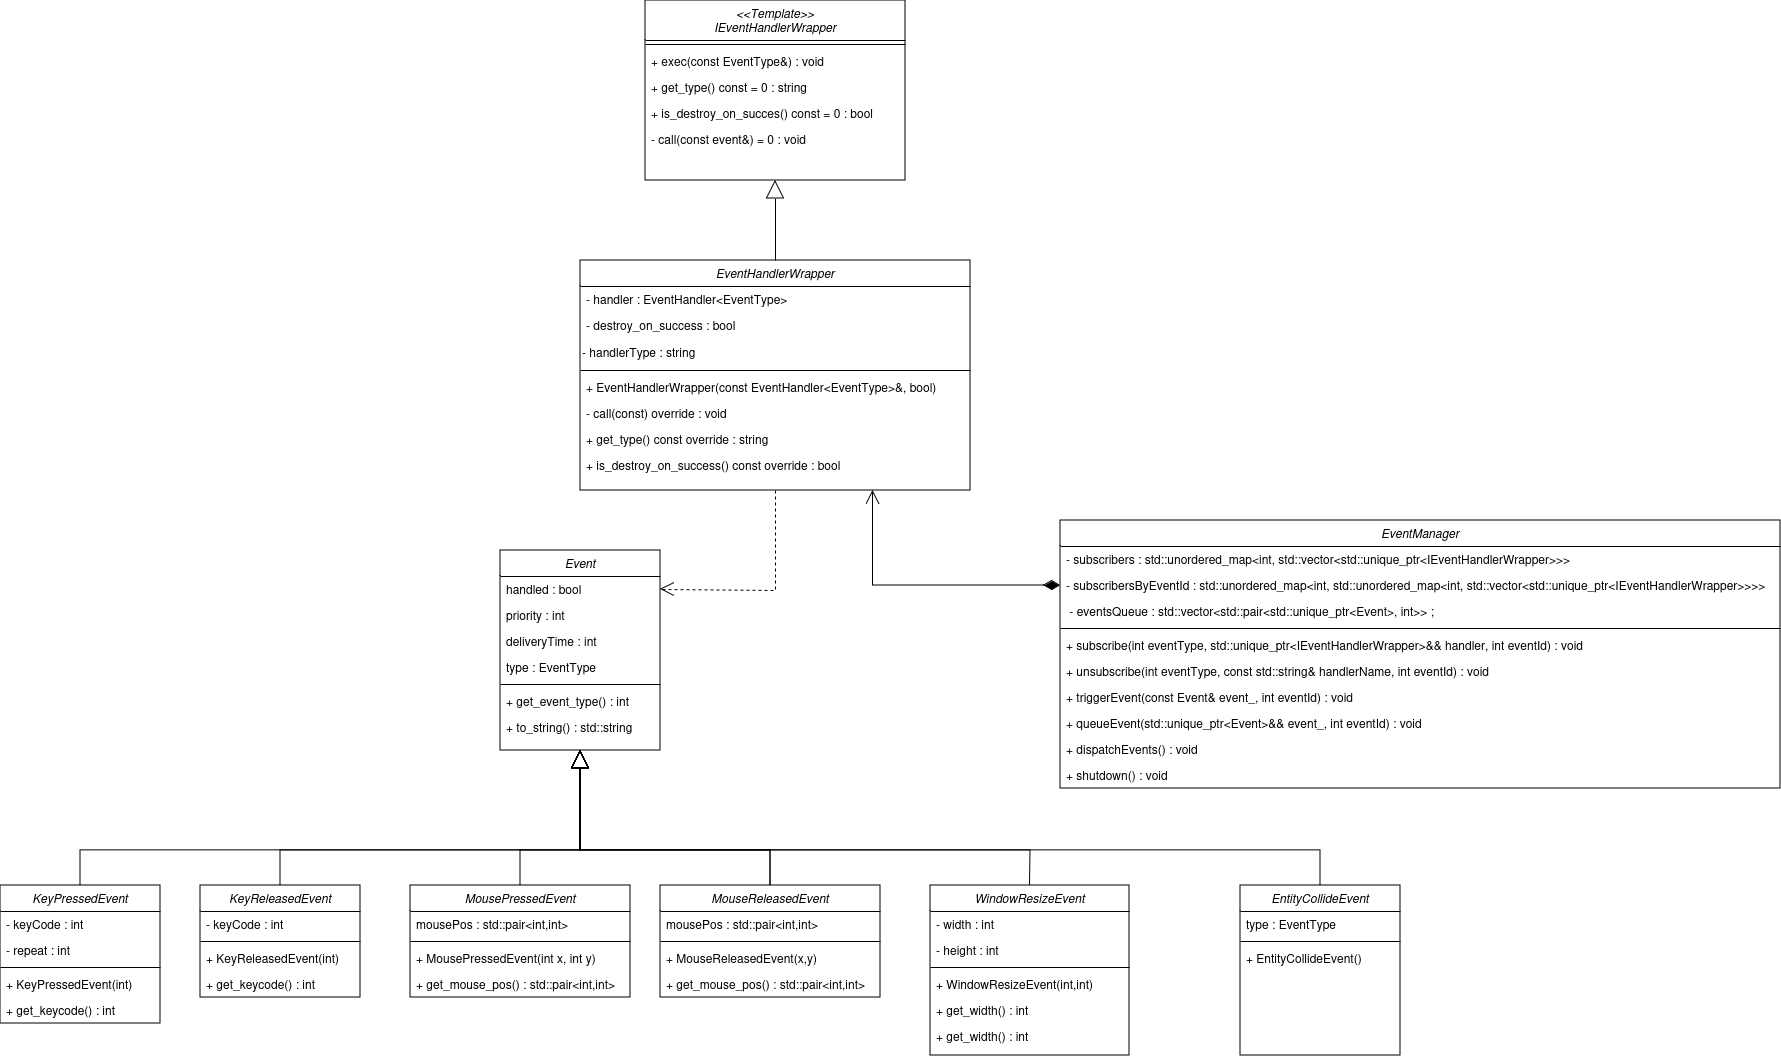
\includegraphics[width=\linewidth]{img/event-uml.drawio.png}  % or specify a custom width
    \caption{event system class diagram}
    \label{fig:event-uml}
\end{figure}
\subsection{Rendering}

\subsection{Physics}

\subsection{Scripting}

The scripting interface was designed around a `target' \gls{api} (described by
\cref{req:script:interface,req:script:user-class,req:script:direct-instance,req:script:direct-run}).
An example of this \gls{api} is shown below:\noparbreak

\begin{blockcode}
class MyScript : public BehaviorScript {
	void update() {
		// update code here
	}
	// init() also exists, but is empty by default
};

{ // in scene initialization
	GameObject & obj = ...;
	obj.add_component<MyScript>();
}
\end{blockcode}

The above call to \codeinline{GameObject::add_component} cannot work correctly
without significantly increasing the complexity of the component manager, so the
following restrictions were taken into account when creating the script system
architecture:\noparbreak

\begin{itemize}
	\item The first template parameter passed to \codeinline{GameObject::add_component}
		\emph{must} be a base `script \emph{component}' class, so each derived user
		script class is instantiated in the same generic script list.
	\item C++ does not allow passing types (i.e.~\codeinline{MyScript} in this case) as
		function parameters, so a function call like
		\codeinline{add_component<BehaviorScript>(MyScript)} cannot be realized.
\end{itemize}

\subsubsection{Architecture}

The restrictions detailed at the start of this section are mitigated as
follows:\noparbreak

\begin{itemize}
	\item User scripts are split into two classes---
		\begin{enumerate}
			\item a script \emph{interface} class (\codeinline{Script})
			\item a script \emph{component} class (\codeinline{BehaviorScript})
		\end{enumerate}
	\item \codeinline{GameObject::add_component} receives the script \emph{component}
		as template parameter
	\item \codeinline{GameObject::add_component} now always returns a reference to the
		component instance
	\item The script component class has a setter function that takes a template
		parameter for classes derived from the base script \emph{interface} class
\end{itemize}

\Cref{fig:class-scripts} shows the resulting structure as a class diagram. It
contains the following classes:\noparbreak
\begin{description}
	\item[Script] This is the script \emph{interface}, and is used by the game
		programmer to create derived script classes. All methods in this class are
		declared virtual and have an empty implementation.

		This class' methods are protected by default, and a friend relation to
		\codeinline{ScriptSystem} is used to ensure only \codeinline{ScriptSystem} is
		able to call these methods.

		Only classes derived from \codeinline{Script} can be used with
		\codeinline{BehaviorScript::set_script}'s template parameter \codeinline{T}. This
		function returns a reference to the \codeinline{BehaviorScript} instance it was
		called on so it can be chained after the call to
		\codeinline{GameObject::add_component}.
	\item[BehaviorScript]
		This is the script \emph{component}, and is given as the template parameter to
		\codeinline{GameObject::add_component}.

		This class also uses a friend relation to \codeinline{ScriptSystem} to restrict
		access to its private reference member \codeinline{script}.
	\item[ScriptSystem] This is the system class that runs the methods implemented in
		the derivative instances of \codeinline{Script}.
\end{description}

\begin{figure}
	\centering
	\includepumldiag{img/class-scripts.puml}
	\caption{User script class diagram}
	\label{fig:class-scripts}
\end{figure}

\subsection{Audio}

Since writing a custom real-time audio mixing engine is outside the scope of this
project\mref and C++ does not provide a built-in cross-platform audio \gls{api}, the
audio system inside the cr\^epe engine is implemented as a fa\c{c}ade around an
existing audio library.

\subsubsection{Libraries}
\label{sec:audio:libs}

This subsection compares various standalone audio libraries for suitability. After
searching for libraries (search terms: `dynamic/adaptive audio', `real-time audio',
`audio library', `game audio engine'), several libraries were found. These libraries
were checked against the audio engine requirements \autocite{crepe:requirements} and
then tested by writing the same benchmark-style \gls{poc} using the remaining
qualifying libraries:\noparbreak
\begin{enumerate}
	\item Load a background track (Ogg Vorbis)
	\item Load three short samples (WAV)
	\item Start the background track
	\item Play each sample sequentially while pausing and resuming the background track
	\item Play all samples simultaniously
	\item Stop all audio and exit
\end{enumerate}

Of these libraries the following were determined to be unsuitable for use in this
project:\noparbreak
\begin{description}
	\item[FMOD \autocite{lib:fmod}] Is proprietary (violates \cref{req:lib:license}).
	\item[PortAudio \autocite{lib:portaudio}] Does not handle mixing.
	\item[miniaudio \autocite{lib:miniaudio}] Tested by implementing a \gls{poc}, but
		dropped due to very limited codec support (WAV, MP3 and FLAC only); Also does not
		have an \gls{api} reference (only programming manual).
	\item[YSE \autocite{lib:yse}] Attempted to write \gls{poc}, but CMake configuration
		in repository is broken; This project seems to have been abandoned.
\end{description}

The only library that remained after these tests is SoLoud \autocite{lib:soloud}. It
is Zlib/LibPng licensed and provides a high-level object-oriented C++ \gls{api}.
\Cref{sec:audio:architecture} describes the fa\c{c}ade written for this library.

\subsubsection{Architecture}
\label{sec:audio:architecture}

\Cref{fig:class-audio-facade} shows a class diagram of the audio fa\c{c}ade. It
contains the following classes:
\begin{description}
	\item[SoundContext] This is a wrapper around the \codeinline{SoLoud::soloud}
		`engine' class, and is therefore implemented as a singleton. This ensures the
		audio engine is initialized before \codeinline{Sound} is able to use it.

		This class is friends with \codeinline{Sound}, so only \codeinline{Sound} is able
		to get the \codeinline{SoundContext} instance.
	\item[Sound] This is a wrapper around the \codeinline{SoLoud::Wav} class, and uses
		cr\^epe's \codeinline{Asset} class to load an audio sample instead.
\end{description}

\begin{figure}
	\centering
	\includepumldiag{img/facade-audio.puml}
	\caption{Audio fa\c{c}ade class diagram}
	\label{fig:class-audio-facade}
\end{figure}

\subsection{Input}

\subsection{Physics}


\section{Tools}

\section{Conclusion}

\end{document}

